\documentclass[12pt, a4paper]{exam}
\usepackage{graphicx}
\usepackage[left=0.8in, top=0.7in, total={6.2in,10in}]{geometry}
\usepackage[normalem]{ulem}
\usepackage{comment}
\usepackage{hyperref}
\usepackage{float}

\renewcommand\ULthickness{1.0pt}   %%---> For changing thickness of underline
\setlength\ULdepth{1.3ex}%\maxdimen ---> For changing depth of underline

\begin{document}
	%\thispagestyle{empty}
	\noindent
	\begin{minipage}[l]{0.1\textwidth}
		\noindent
		
\includegraphics[width=1.8\textwidth]{res/iiserb_logo.png}
	\end{minipage}
\hfill
\begin{minipage}[c]{0.8\textwidth}
	\begin{center}
		{\large	Indian Institute of Science Education and Research Bhopal \par
		\large	\par
	\large \textbf{	Computer Vision(DSE-312/EECS-320)}	\par
\small	Assignment-2}
	\end{center}
\end{minipage}

\par
\vspace{0.2in}
\noindent
\textbf{Name: }Adheesh Trivedi\\
\noindent
\textbf{Roll No.:  }22016\\
\noindent
\uline{\textbf{Time of submission: } \hfill 		\hfill Marks Obtained: } \\
\uline{Please follow the instructions given in the assignment carefully.}
\par 
\vspace{0.15in}
\noindent
\centering
{\small \bfseries
\begin{enumerate}
    \item All questions are mandatory. Plagiarism and copying from anywhere (similar
    submission) can debar you from this course and invite the academic dishon-
    esty policy.
    \item Implement all algorithms purely in Python without using specialized libraries
    like OpenCV or PIL for the processing. You may use libraries for basic
    operations (like loading an image), but the algorithms should be coded from
    scratch.
    \item Comment on your code extensively to explain your logic and the steps you
    are implementing.
    \item Display both the original and processed images to compare results.
    \item Make a short 7-minute video and explain your code.
    \item A report reflecting on what you have learned. Visualization of the output
    must be there along with other necessary details.
\end{enumerate}
}

\vspace{0.2in}
\begin{questions}
	\pointsdroppedatright
	\question

Apply the filters mentioned below on the image attached and analyze their impact.
Describe what you found after applying each filter and why certain phenomena
occur. \textbf{\textit{(Marks:6)}}
\begin{itemize}
    \item SIFT
    \item Bag of Words
    \item HOG
\end{itemize}

\begin{figure}[H]
    \centering
    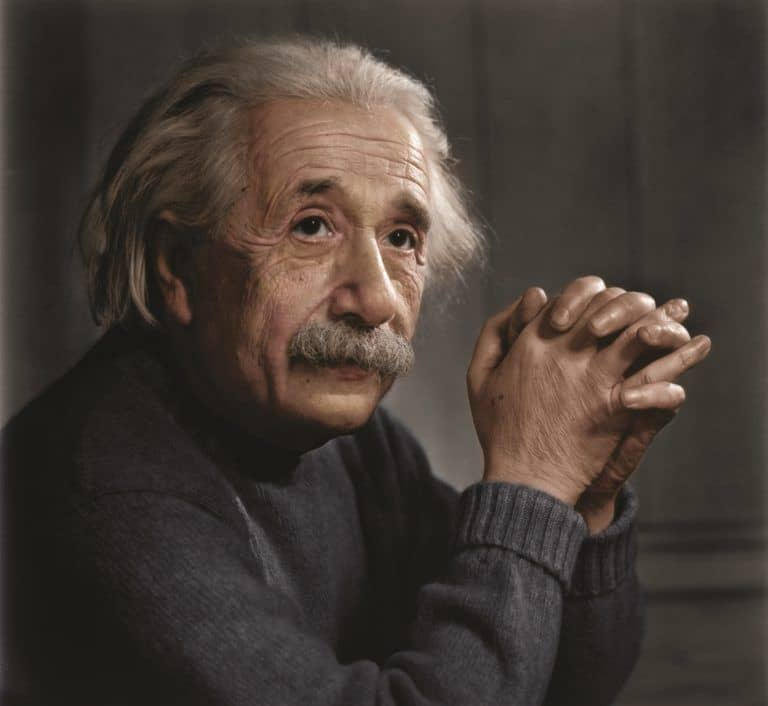
\includegraphics[width=.3\textwidth]{res/Albert_Einstein.jpg}
    \caption{Image of Albert Einstein}
    \label{fig:1q}
\end{figure}

\vspace{0.2in}
	\pointsdroppedatright 
\textbf{Answer:}

I used the $3\times3$ Prewitt filter to produce image dipicting the edges in the original image:

$$\delta_x = \frac{1}{3}
\begin{bmatrix}
    -1 & 0 & 1 \\
    -1 & 0 & 1 \\
    -1 & 0 & 1
\end{bmatrix}$$

and,

$$\delta_y = \frac{1}{3}
\begin{bmatrix}
-1 & -1 & -1 \\
0 & 0 & 0 \\
1 & 1 & 1
\end{bmatrix}$$

These filters when convolved with the original image gives the following images:

\begin{figure}[H]
    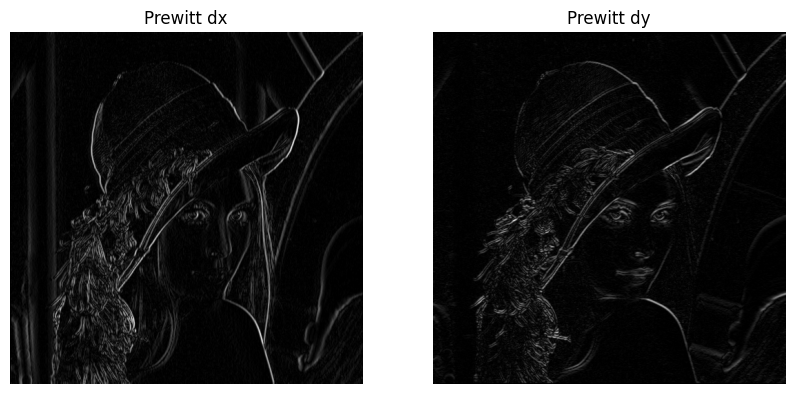
\includegraphics[width=1.06\textwidth]{res/1_prewitt.png}
    \caption{Prewitt filter applied to the original image}\label{fig:1_prewitt}
\end{figure}

Here we notice that the images is highlighting the edges that were in the orignial image.

\textbf{Comparision with larger filter (5 by 5)}

I used the following $5\times5$ filter to produce image dipicting the edges in the original image:

$$\delta_x = \frac{1}{15}
\begin{bmatrix}
-1 & -2 & 0 & 2 & 1 \\
-1 & -2 & 0 & 2 & 1 \\
-1 & -2 & 0 & 2 & 1 \\
-1 & -2 & 0 & 2 & 1 \\
-1 & -2 & 0 & 2 & 1
\end{bmatrix}$$

and,

$$\delta_y = \frac{1}{15}
\begin{bmatrix}
-1 & -1 & -1 & -1 & -1 \\
-2 & -2 & -2 & -2 & -2 \\
0 & 0 & 0 & 0 & 0 \\
2 & 2 & 2 & 2 & 2 \\
1 & 1 & 1 & 1 & 1
\end{bmatrix}$$

Here the 2nd and 2nd last enteries have greater value than the first and the last enteries. This is because the center pixel has more weightage than the pixels at the corners. This is done to increase localization in the gradient.

\begin{figure}[H]
    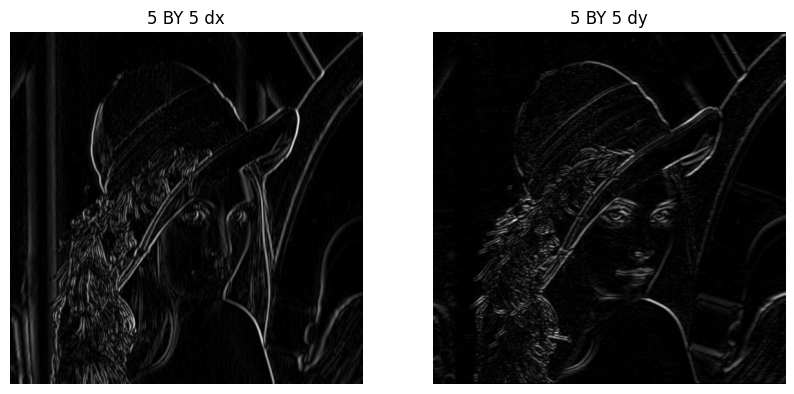
\includegraphics[width=1.06\textwidth]{res/1_5_by_5.png}
    \caption{5 by 5 filter applied to the original image}\label{fig:1_5by5}
\end{figure}

\textbf{Results}

The $\delta_x$ filter detects vertical edges and the $\delta_y$ filter detects horizontal edges. This is happening because the filter computes gradient about the direction mentioned in its subscript. So when there is sudden change in the pixel values in the direction of the filter, the filter gives a high value. Since edges are nothing but sudden changes in a function. This is why the edges are highlighted in the images.

Few differences observed between different size of filters:

\begin{itemize}
    \item The edges are thicker in $5\times5$ than in $3\times3$.
    \item $3\times3$ does a lot better in preserving the hair details.
\end{itemize}

\newpage
\question

Imagine you’re monitoring pedestrian movement at a crosswalk. Your task is to track the direction and speed of pedestrians in a video using optical flow analysis. Use OpenCV’s built-in video vtest.avi, which simulates real-world pedestrian movement. \textbf{\textit{(Marks: 6 )}}

\begin{itemize}
    \item Using the Lucas-Kanade method, track specific points in the video to capture the movement of pedestrians.
    \item Visualize the direction of movement using arrows to indicate the flow direction at each point.
    \item Provide a brief summary: What patterns do you observe in pedestrian movement? Are there any areas where pedestrians tend to cluster or move faster?
\end{itemize}
\vspace{0.2in}
	\pointsdroppedatright 
\textbf{Answer:}

\textbf{Loading dataset}

I loaded 500 images of real faces and 500 images of spoof faces from the dataset.

\textbf{Raw pixel values}

The raw pixel values of the face images are used as features. I trained a Support Vector Machine (SVM) classifier on these raw pixel features to classify fake and real faces. The performance of the model on the dataset is portrayed in the code.

\textbf{Local Binary Patterns (LBP) features}

Local Binary Patterns (LBP) features are extracted from the face images for feature extraction. I trained an SVM classifier using the LBP features to classify fake and real faces. The performance of the model on the dataset is portrayed in the code.

\begin{figure}[H]
    \centering
    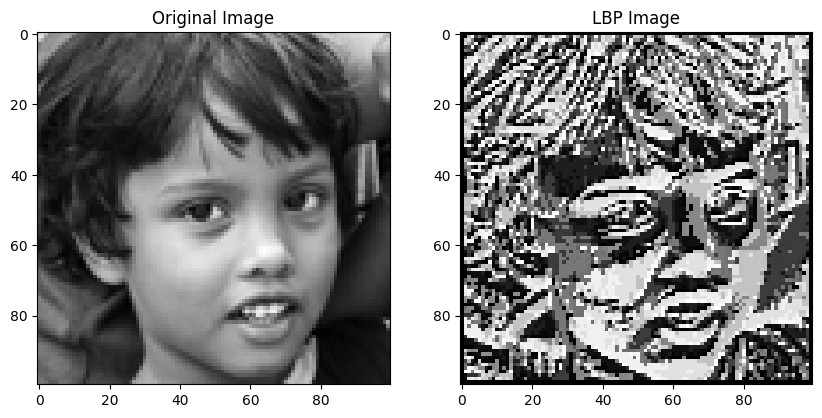
\includegraphics[width=.9\textwidth]{imgs/lbp.png}
    \caption{Local binary pattern}
    \label{fig:2_mediapipe}
\end{figure}

\newpage

\textbf{Edge methods}

Edge images are computed using the Prewitt and Sobel edge detectors. These edge images are used as input features independently to train an SVM classifier and classify fake and real faces. The performance of the model on the dataset is portrayed in the code.

\begin{figure}[H]
    \centering
    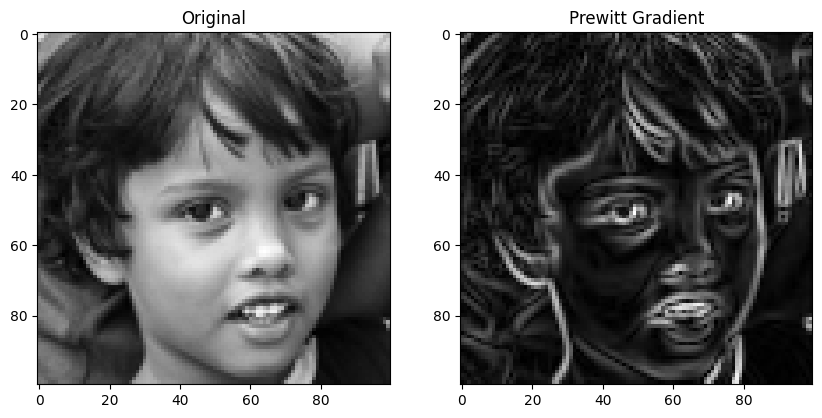
\includegraphics[width=.9\textwidth]{imgs/prewitt.png}
    \caption{Prewitt filtered image}
    \label{fig:2_mediapipe}
\end{figure}


\begin{figure}[H]
    \centering
    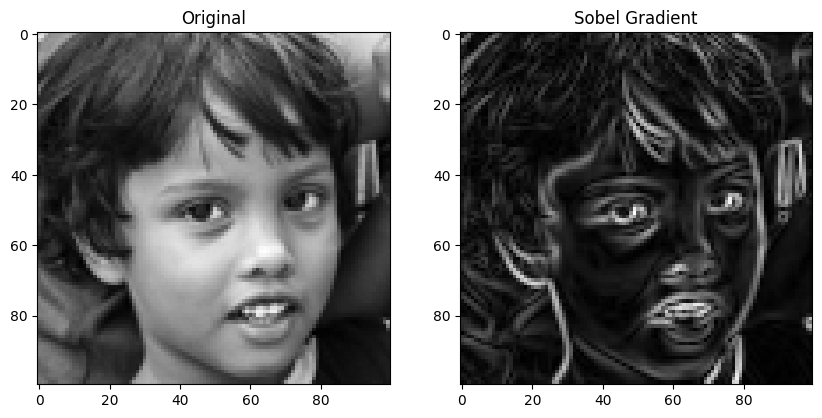
\includegraphics[width=.9\textwidth]{imgs/sobel.png}
    \caption{Sobel filtered image}
    \label{fig:2_mediapipe}
\end{figure}

\end{questions}

\end{document}